% Section content template for individual Educative lessons
% This file contains the actual content for a specific section
% Generated from Educative API section content

% Section: Use Case Diagram for Facebook
% Section ID: 5550076061810688
% Section Slug: use-case-diagram-for-facebook
% Generated: 2025-12-14T12:38:52.373920

Let's begin building Facebook's use case diagram and understanding its components' relationship. First , we will define the different elements of our Facebook system, followed by the complete use case diagram.

\subsection{System}\label{Oa_C_X_Xopu6H6vwg5jFU}
\\
Our system is Facebook.

\subsection{Actors}\label{cMhqlcmVTyx0y510r-UVt}
\\
Now, we'll define the main actors of Facebook.

\subsubsection{Primary actors}\label{EC2WaQXB654ygbo5Yle8i}

\begin{itemize}
\item
\protect\phantomsection\label{HWfbdXLULS5_WG7yJjw8C}
\textbf{User:} This actor can create a personal profile that includes their information. They can create posts, pages, and groups, and interact with other users by sending friend requests and messages, commenting on posts, and more.
\end{itemize}

\subsubsection{Secondary actors}\label{dUzhQ_rbY0yQvMnccxZ3v}

\begin{itemize}
\item
\protect\phantomsection\label{-pJVIPgtSKNq5s6320kp7}
\textbf{Page/Group admin:} The admin is in charge of performing numerous operations, including blocking or unblocking users from groups or pages, deleting an existing group, and changing the group's privacy.
\item
\protect\phantomsection\label{_JSoiFqjoPXA9TrBwWybe}
\textbf{System:} This is responsible for sending notifications for new friend requests, messages, comments, etc.
\end{itemize}

\subsection{Use cases}\label{hTYPmWhIDrxDNBzR3GSsL}
\\
In this section, we'll define Facebook's use cases. We have listed them according to their interactions with a particular actor.
\begin{quote}
\textbf{Note:} Some use cases will occur multiple times because they are shared among different actors in the system.
\end{quote}
\subsubsection{User}\label{OTjnh7B38pHFr7Kvy5xDc}

\begin{itemize}
\item
\protect\phantomsection\label{F_7fYgob8Nd3YIjdgQ84D}
\textbf{Add/update profile:} To add information like work, education, and places of visit details, or to update an existing profile.
\item
\protect\phantomsection\label{JHmr130q4QyXi7RW4WCrg}
\textbf{Follow/unfollow user:} To follow or unfollow other users.
\item
\protect\phantomsection\label{PmQC4TgZ-x9qJxn3DIlja}
\textbf{Send message:} To send a message to other users.
\item
\protect\phantomsection\label{MAqy3CU0ludy3vopAYuDt}
\textbf{Send friend request:} To send a friend request to other users.
\item
\protect\phantomsection\label{CxeknDRlgzzHJw-hUZu2D}
\textbf{Create/like/follow/share page:} To create a new page or perform actions including liking, following, or sharing an existing page.
\item
\protect\phantomsection\label{TZ_i2_Uow9xh6K5LQDQ2f}
\textbf{Create/join/leave group:} To create a new group or perform actions like joining or leaving an existing one.
\item
\protect\phantomsection\label{HsiFbA4PyJ5CYNodXoLAC}
\textbf{Invite users to group:} To invite other users to an existing group.
\item
\protect\phantomsection\label{ZEqjAESY5TIxmsi2UpGcX}
\textbf{Add/update/delete post:} To add a new post, update the post's content, or delete an existing post.
\item
\protect\phantomsection\label{uyiimXdtCr53Du7ZL8V4T}
\textbf{Like/comment/share post}: To like a post, comment on a post, or share a post.
\item
\protect\phantomsection\label{Vpeho-ghM7uk9x2Tu-8dx}
\textbf{Add/update/delete/like comment:} To add a new comment, update the comment's content, like a particular comment, or delete a comment.
\item
\protect\phantomsection\label{3-61Bx2roeRVUQWxABp3W}
\textbf{Accept/reject friend request:} To accept or reject a friend request from another user.
\item
\protect\phantomsection\label{T3Z-bGo2AP2bZwbYAPUpU}
\textbf{Update privacy:} To update the privacy settings of the profile.
\item
\protect\phantomsection\label{8J5gY6h4K13SGLUQAVG-0}
\textbf{Search users/groups/pages/posts:} To search for other users, any existing groups or pages, or any posts made by users.
\item
\protect\phantomsection\label{lp7FNRbMzWnvtz2rqsuHo}
\textbf{Accept/Reject friend request:} To accept or reject a friend request from another Facebook user.
\item
\protect\phantomsection\label{6cIu85rchJJptN0cLCK_P}
\textbf{Accept/Reject group join invitation:} To accept or reject a group joining invitation from another Facebook user.
\item
\protect\phantomsection\label{xL_JTxxHNDlZSMKumrOHJ}
\textbf{Like/Comment/Share post:} To like, comment, or share any post visible to users on Facebook.
\end{itemize}

\subsubsection{Page/Group admin}\label{90gxYT6p4TvDwt3jDunqj}

\begin{itemize}
\item
\protect\phantomsection\label{BQxbKGZrutf4eoBPhhH5o}
\textbf{Block/unblock page user:} To block or unblock a user from a page.
\item
\protect\phantomsection\label{BQxbKGZrutf4eoBPhhH5o}
\textbf{Block/unblock group user:} To block or unblock a user from a group.
\item
\protect\phantomsection\label{S2i2OpLii23Kt_IlOjvfB}
\textbf{Change a group's privacy:} To change the privacy settings of a group (from public to private and vice versa).
\end{itemize}

\subsubsection{System}\label{UHUCT51fVgCEXmtFp9oGP}

\begin{itemize}
\item
\protect\phantomsection\label{g8wQR_WBYDg8GFewcfLCG}
\textbf{Send new friend request notification:} To send a notification of any friend request sent by another user.
\item
\protect\phantomsection\label{7yqOVw48IWZ8re9Jl2iPR}
\textbf{Send message notification:} To send a notification of any new messages.
\item
\protect\phantomsection\label{rHE_Rs62f21YXq_FTzfjA}
\textbf{Send new post notification:} To send a notification of any new posts.
\item
\protect\phantomsection\label{2EHlRvv3wcajt4ULCZpcx}
\textbf{Send comment notification:} To send a notification of any comments on your or others' posts.
\end{itemize}

\subsection{Relationships}\label{XQvggC3T4Ugq5zdQ2BHLs}
\\
This section describes the relationships between and among actors and their use cases.

\subsubsection{Generalization}\label{IxW9YTLIvU8ZpZHgoEimO}

\begin{itemize}
\item
\protect\phantomsection\label{qqgOqRcw5qDnU9cVfWzjr}
The ``Page/Group admin'' has a generalization relationship with the ``User'' as the admin can perform all the tasks a normal user can perform.
\end{itemize}

\subsubsection{Associations}\label{vK-QfWjvcDlR4kxAtjyB2}
\\
The table below shows the association relationship between actors and their use cases.

\begin{table}[htbp]
\centering
\small
\adjustbox{max width=\textwidth}{
\begin{tabular}{|p{0.316\textwidth}|p{0.325\textwidth}|p{0.308\textwidth}|}
\hline
\textbf{User} & \textbf{Page/Group Admin} & \textbf{System} \\
\hline
\hline
Add/update profile & Block/unblock page user & Send new friend request notification \\
\hline
Follow/unfollow user & Enable/disable group user & Send message notification \\
\hline
Send message & Change a group's privacy & Send new post notification \\
\hline
Send friend request & \hfill\break & Send comment notification \\
\hline
Create/like/follow/share page & \hfill\break & \hfill\break \\
\hline
Create/join/leave group & \hfill\break & \hfill\break \\
\hline
Invite user to group & \hfill\break & \hfill\break \\
\hline
Add/update/delete post & \hfill\break & \hfill\break \\
\hline
Add/update/delete/like comment & \hfill\break & \hfill\break \\
\hline
Accept/reject friend request & \hfill\break & \hfill\break \\
\hline
Update privacy & \hfill\break & \hfill\break \\
\hline
Search users/groups/pages/posts & \hfill\break & \hfill\break \\
\hline
Accept/Reject friend request & \hfill\break & \hfill\break \\
\hline
Accept/Reject group join invitation & \hfill\break & \hfill\break \\
\hline
Like/Comment/Share post & \hfill\break & \hfill\break \\
\hline
\hfill\break & \hfill\break & \hfill\break \\
\hline
\end{tabular}
}
\end{table}

\subsubsection{Include}\label{E6c3ykAkGs3AZ07d6dOGz}

\begin{itemize}
\item
\protect\phantomsection\label{ANyTU2AprtuNrjUDmxAeR}
When a user takes an action that triggers a notification to others---such as sending a friend request, message, posting, or commenting---the system notifies the relevant users. These are best represented using ``include'' relationships:

\begin{itemize}
\item
The \textbf{Send friend request}, \textbf{Send message}, \textbf{Add post}, and \textbf{Add comment} use cases all include their respective notification use cases:

\begin{itemize}
\item
The \textbf{Send friend request} use case includes the \textbf{Send new friend request notification} use case.
\item
The \textbf{Send message} use case includes the \textbf{Send message notification} use case.
\item
The \textbf{Add post} use case includes the \textbf{Send new post notification} use case.
\item
The \textbf{Add comment} use case includes the \textbf{Send new comment notification} use case.
\end{itemize}
\end{itemize}
\item
\protect\phantomsection\label{YPyqnO0Jh6JtXPtY7ZSQn}
When a user updates their profile, they may modify work experience, education, or place of residence.

\begin{itemize}
\item
The \textbf{Update profile} use case includes the \textbf{Add/update work}, \textbf{Add/update education}, and \textbf{Add/update place} use cases.
\end{itemize}
\item
\protect\phantomsection\label{Fqc0LCbM_qrtthNVxiDlc}
When a user performs a search, the system performs sub-searches across multiple categories.

\begin{itemize}
\item
The \textbf{Search} use case includes the \textbf{Search Users}, \textbf{Search Groups}, \textbf{Search Pages}, and \textbf{Search Posts} use cases.
\end{itemize}
\end{itemize}

\subsection{Use case diagram}\label{7ouMipsMGCTcgsiA94UDU}
\\
Here's the use case diagram of Facebook:

\begin{figure}[htbp]
 \centering
 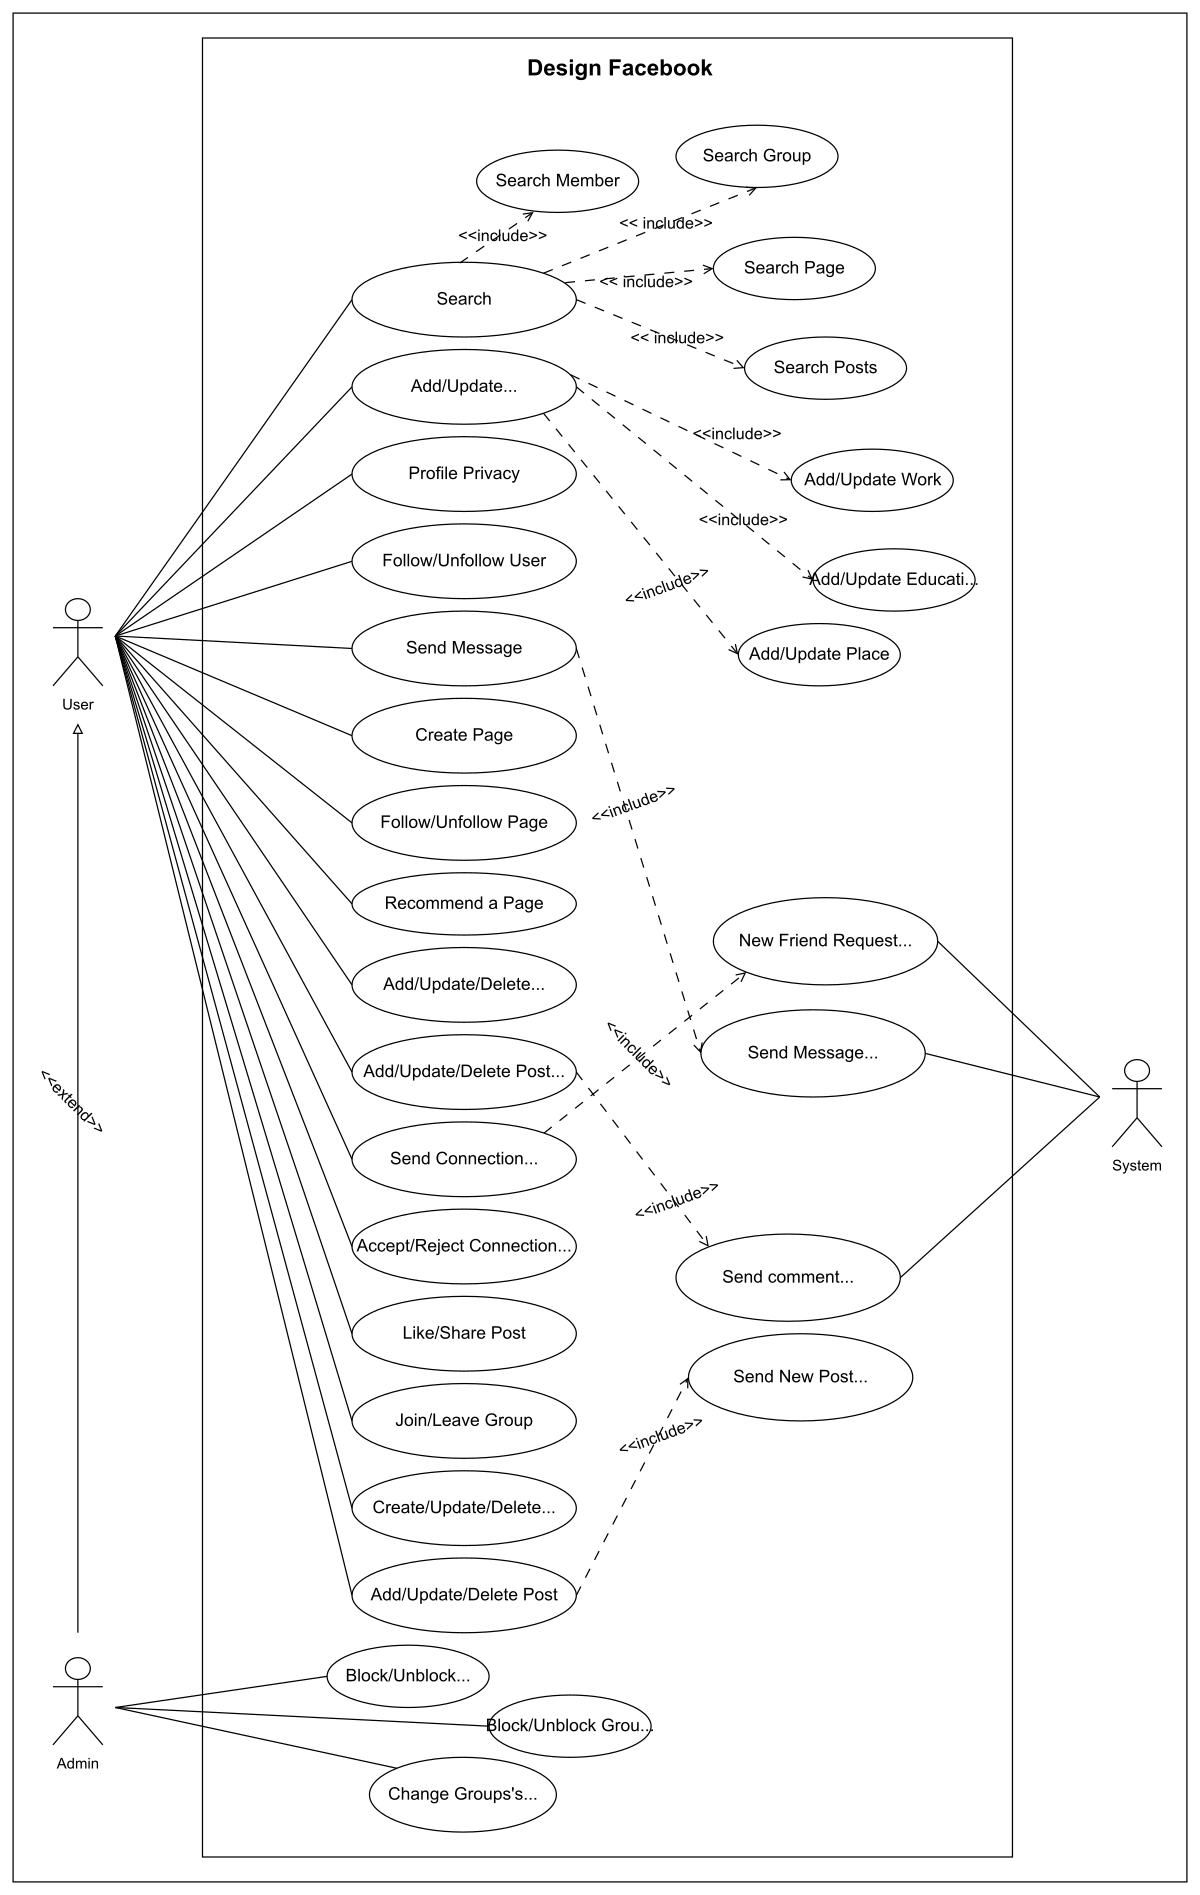
\includegraphics[width=0.5\textwidth]{Images/chapter_22/section_5550076061810688/4826687727337472.png}
 \caption{The use case diagram of Facebook}
\end{figure}

In the next lesson, we will discuss the class diagram with a detailed explanation of all classes and their relationship with each other.

% End of section content